% Created: Enze Chen, July 2017
% Last edited: Enze Chen, December 2017
%
% Chapter 8 of the MSE 142 coursereader. This chapter discusses time-dependent perturbation theory. The various approximations for the probability amplitudes are discussed, and particular focus is drawn to sinusoidal perturbations. These model electric fields, which can be applied to stimulated emission in lasers.

% Uncomment the following three lines and last line to individually compile this chapter
%\documentclass[12pt, english]{book}
%\usepackage{142crstyle}
%\begin{document}

\chapter[Perturbation Theory]{Time-dependent Perturbation Theory} \label{ch:pert}
%{ \doublespacing 
For the final topic covered in this text, we would like to understand the interaction of light with matter---how materials absorb light, emit light, and the basic ideas behind the operation of the laser. Much of the phenomenon here can be explained using QED, but for the sake of simplicity we will return to the single-particle wave functions used in first quantization. However, one of the key differences between these interactions and our previous examples is that our Hamiltonian is now time-dependent, so instead of solving for a stationary state we must now solve for a superposition state. This framework allows us to model atomic transitions between energy levels due to the emission or absorption of radiation by an atom.

\section{General formalism}
To start off, let's suppose we have a quantum system with known Hamiltonian $H_0(r)$\footnote{We use $r$ here to represent the position vector, which you can view equivalent to $x$.} which we have already solved the \Sch\ equation for, i.e.
\begin{equation*}
	H_0\Psi_n = i\hbar \pdv{\Psi_n}{t}
\end{equation*}
with stationary state solutions
\begin{equation*}
	\Psi_n(r,t) = \psi_n(r)e^{-iE_nt/\hbar}
\end{equation*}

We can now apply a small perturbation $H'(r,t)$ of strength $\lambda$ such that the total Hamiltonian becomes 
\begin{tcolorbox}[title = Hamiltonian for small perturbations] \vspace{-2ex}
	\begin{equation}
	\hat{H}(r,t) = H_0(r) + \lambda H'(r,t) \label{eq:ham-pert}
	\end{equation}	
\end{tcolorbox}
	
where all of the time-dependence is accounted for by the second term. Here, $\lambda \ll 1$ characterizes the strength of the perturbation. As we will see, the problem becomes too difficult to solve in general for arbitrary $\lambda$, but in the case when $\lambda$ is small, we can develop a simple approximate theory. The theory will be quite general---only at the end will we apply it to specific examples associated the interactions between light and matter. In any case, the time-dependent \Sch\ equation that we are now trying to solve becomes
\begin{equation}
	\left(H_0 + \lambda H'\right)\Psi = i\hbar \pdv{\Psi}{t} \label{eq:sch-pert}
\end{equation}

Since this general equation is impossible to solve exactly, we will employ the method of \textbf{eigenfunction expansion}, which you've already seen for the particle in a box. We expand the general solution $\Psi(r,t)$ we are trying to find in terms of the known solutions of $H_0$:
\begin{equation}
	\Psi(r,t) = \sum_n c_n(t) \Psi_n(r,t) \label{eq:exp-pert}
\end{equation}
where the individual states $\Psi_n$ are orthonormal basis vectors. This again corresponds to a quantum superposition state with $c_n(t)$ the amplitude of each state in the superposition and $\abs{c_n(t)}^2$ the probability that a measurement finds the system in state $n$ at time $t$ (technically that a measurement of the energy will return $E_n$). Since we are trying to solve for the case where there is only a slight perturbation to the known Hamiltonian, it's a good guess to try to find solutions which can be expressed in terms of the known solutions of $H_0$. Our goal will be to find a general equation for the $c_n$'s, since the probability amplitudes are now changing in time. Once we know these, we know the full time-dependent evolution of the wave function. \par 

%%%%%%%%%%%%%%%%%%%%%%%%%%%%%%%%%%%%%%%%%%%%%%%%%%%%%%%%%%%%%%%%%%%%%%%%%%%%%%%%

\subsection{Probability amplitude}
If we substitute the expansion in Equation~\ref{eq:exp-pert} into our time-dependent \Sch\ equation, we find
\begin{align*}
	\left(H_0 + \lambda H'\right)\Psi &= i\hbar \pdv{\Psi}{t} \\
	H_0 \sum_n c_n(t) \Psi_n(r,t) + \lambda H'\sum_n c_n(t) \Psi_n(r,t) &= i\hbar \pdv{t}\sum_n c_n(t) \Psi_n(r,t) \\
	i\hbar\sum_n c_n(t) \pdv{\Psi_n}{t} + \lambda H'\sum_n c_n(t) \Psi_n(r,t) &= i\hbar \sum_n c_n(t) \pdv{\Psi_n}{t} + i\hbar \sum_n \dv{c_n(t)}{t} \Psi_n(r,t) \\
	\lambda H'\sum_n c_n(t) \Psi_n(r,t) &= i\hbar \sum_n \dot{c}_n(t) \Psi_n(r,t)
\end{align*}

In the last line we used dot notation to represent the time derivative of a quantity, such that $\dot{c_n}=\dv{c_n}{t}$. We take the last line and multiply both sides on the left with $\bra{\Psi_k}$ to obtain
\begin{equation*}
	\lambda \sum_n c_n \braket{\Psi_k}{H'\Psi_n} = i\hbar \sum_n \dot{c}_n \braket{\Psi_k}{\Psi_n}
\end{equation*}

Why is this useful? Because we claimed that the stationary state solutions were orthogonal, this allows us to pick out just one term in the sum on the right hand side, namely the term with $k=n$. All the other terms are zero. Thus, the final equation we find is
\begin{tcolorbox}[title = Relationship for $c_k$] \vspace{-2ex}
	\begin{equation}
		i\hbar \dot{c}_k = \lambda \sum_n c_n H_{kn}' \label{eq:cdot}
	\end{equation}
\end{tcolorbox}

Here, $H_{kn}' = \braket{\Psi_k}{H'\Psi_n}$. These are typically called \textbf{matrix elements} because the perturbing Hamiltonian is a matrix operator and we are interested in the element in the $k$th row and $n$th column of this matrix. Equation~\ref{eq:cdot} is an infinite series of coupled differential equations and not so easy to deal with. But so far, we have been completely general, i.e. we have not made use of the fact that we are trying to solve for the case of a small perturbation. To do this, we guess the solution
\begin{equation}
	\boxed{c_k(t) = c_k^{(0)} + \lambda c_k^{(1)}(t) + \lambda^2 c_k^{(2)}(t) + \cdots} \label{eq:c-pow}
\end{equation}
which we obtained by expanding $c_k(t)$ in a \textbf{power series in} $\lambda$. The superscript in parentheses indicates the order of the approximation for $c_n$. Again, this is a reasonable assumption in the limit when $\lambda$ is small.\footnote{This is largely a convergence argument, and a brief explanation is given by \href{http://tutorial.math.lamar.edu/Classes/CalcII/PowerSeriesandFunctions.aspx}{Paul Dawkins}.} In the following, what we'll do is find an equation for the first order correction term $c_k^{(1)}$. If we substitute the above equation into both sides of Equation~\ref{eq:cdot} and equate powers of $\lambda$ (since $\lambda$ is arbitrary, those terms with the same power must be equal), we obtain the following equations:
\begin{align}
	i\hbar \dot{c}_k^{(0)} &= 0 \label{eq:cdot0} \\
	i\hbar \dot{c}_k^{(1)} &= \sum_n H_{kn}' c_n^{(0)} \label{eq:cdot1} \\
	&\vdots \nonumber \\
	i\hbar \dot{c}_k^{(n)} &= \sum_n H_{kn}' c_n^{(n-1)} \label{eq:cdotn}
\end{align}

So, if we can find $c_k^{(0)}$, we can use this to find $c_k^{(1)}$, then $c_k^{(2)}$, and so on. \par 

As an example, let's assume at time $t=0$, the system is sitting in a stationary state of $H_0$, say $\Psi_l$, such that
\begin{equation*}
	\Psi(r,t)|_{t=0} = \Psi_l(r,t) = \sum_n c_n(t) \Psi_n(r,t)
\end{equation*}

So what is $c_n^{(0)}$? Well, the summation runs over state $l$, so it must be the case that all the $c_n$'s are zero except when $n=l$, in which case $c_l=1$. This can be written simply in terms of the \textbf{Kronecker delta function} as
\begin{equation}
	c_n^{(0)} = \delta_{n,l}
\end{equation}
which is 0 if $n\neq l$ and 1 if $n=l$.\footnote{The Kronecker delta function is analogous to the Dirac delta function, just applied to discrete arguments.} So now we have $c_k^{(0)}$ as set by the initial conditions and we can solve for the first order correction term. Using Equation~\ref{eq:cdot1}, 
\begin{equation}
	i\hbar \dot{c}_k^{(1)} = \sum_n H_{kn}' \delta_{n,l} = H_{kl}'
\end{equation}

which leads to
\begin{tcolorbox}[title = First order perturbation coefficient] \vspace{-2ex}
	\begin{equation}
		c_k^{(1)}(t) = \frac{1}{i\hbar} \int_{0}^{t_0} H_{kl}'(r,t) \dd{t} \label{eq:c1}
	\end{equation}
\end{tcolorbox}

The square of this quantity gives the probability of making an atomic transition from state $\Psi_l$ to state $\Psi_k$ after some time $t_0$, at least to first order. If higher accuracy is required, we can easily write down the equation for the second order approximation as follows:
\begin{equation*}
	i\hbar \dot{c}_k^{(2)} = \sum_{m\neq l} H_{km}'c_m^{(1)}
\end{equation*}

Inserting Equation~\ref{eq:c1} into the right hand side and taking the integral, we get
\begin{equation}
	c_k^{(2)} = -\frac{1}{\hbar^2} \sum_{m\neq l} \int_{t'}^{t_0} H_{km}'(r,t) \left[ \int_{0}^{t'} H_{ml}'(r,t) \dd{t} \right] \dd{t}
\end{equation}

Of course, we could theoretically continue doing these successive approximations to get higher order corrections and more accurate calculations of $c_k(t)$. The second order approximation allows us to model an intermediate transition from $\Psi_l$ to some state $\Psi_m$ and then finally to $\Psi_k$. In most cases, of course, the first order approximation is sufficient, and certainly in our case as a pedagogical example of the theory.\footnote{Now unless otherwise stated, assume $c_k(t)$ refers to the first order approximation $c_k^{(1)}(t)$ because we set $c^{(0)}_{j \neq l} = 0$.}

%%%%%%%%%%%%%%%%%%%%%%%%%%%%%%%%%%%%%%%%%%%%%%%%%%%%%%%%%%%%%%%%%%%%%%%%%%%%%%%%

\subsection{Separation of variables}
Before we get to the application of this theory, let's take a closer look at Equation~\ref{eq:c1}. One can often factor the perturbation Hamiltonian as $H'(r,t) = \bar{H}'(r)f(t)$, in which case the matrix element $H'_{kl}$ can be written as
\begin{align*}
	H'_{kl} &= \braket{\Psi_k}{H'\Psi_l} \\
	&= f(t) \braket{\psi_ke^{-iE_kt/\hbar}}{\bar{H}'\psi_le^{-iE_lt/\hbar}} \\
	&= f(t) \braket{\psi_k}{\bar{H}'\psi_l}e^{i(\omega_k-\omega_l)t} \\
	&= f(t) \bar{H}'_{kl} e^{i\omega_{kl}t} 
\end{align*}

where we have defined a new matrix element $\bar{H}'_{kl}$ and the quantity $\omega_{kl} = \omega_k - \omega_l = (E_k - E_l)/\hbar$. Note that the matrix element is in principle easy to calculate, at least numerically. We know the solutions of the unperturbed Hamiltonian and therefore can calculate this integral for arbitrary $k$ and $l$. We then have another form of Equation~\ref{eq:c1} for the time-dependent amplitude:
\begin{equation}
	\boxed{c_k(t) = \frac{\bar{H}'_{kl}}{i\hbar} \int_{0}^{t_0} e^{i\omega_{kl}t} f(t) \dd{t}} \label{eq:c1-sep}
\end{equation}

The first order approximation of the probability of the system making a transition from an initial state $l$ to state $k$ is therefore
\begin{tcolorbox}[title = Transition probability] \vspace{-2ex}
	\begin{equation}
		P_{l \rightarrow k} = \abs{c_k}^2 = \abs{\frac{\bar{H}'_{kl}}{\hbar}}^2 \abs{\int_{0}^{t} e^{i\omega_{kl}t'} f(t') \dd{t'}}^2
	\end{equation}
\end{tcolorbox}

This is the fundamental result that we will apply in the next section.

%%%%%%%%%%%%%%%%%%%%%%%%%%%%%%%%%%%%%%%%%%%%%%%%%%%%%%%%%%%%%%%%%%%%%%%%%%%%%%%%

\section{Sinusoidal perturbation}
As a simple application of the previous equation for the transition probability, let's suppose that at time $t<0$ the atom is in a stationary state $l$. Starting at $t=0$, we apply a monochromatic electromagnetic wave that gives a sinusoidal perturbation $H'(r,t) = 2H'(r)\cos(\omega t)$. Substituting this expression into Equation~\ref{eq:c1-sep}, we find
\begin{align*}
	c_k(t) &= \frac{H'_{kl}}{i\hbar} \int_{0}^{t_0} e^{i\omega_{kl}t} \left( 2\cos(\omega t) \right) \dd{t} \\
	&= \frac{H'_{kl}}{i\hbar} \int_{0}^{t_0} e^{i\omega_{kl}t} \left(e^{i\omega t} + e^{-i\omega t} \right) \dd{t} \\
	&= \frac{H'_{kl}}{i\hbar} \int_{0}^{t_0} e^{i(\omega_{kl}+\omega)t} + e^{i(\omega_{kl}-\omega)t} \dd{t} \\
	&= -\frac{H'_{kl}}{\hbar} \left[ \frac{e^{i(\omega_{kl}+\omega)t}}{\omega_{kl}+\omega} + \frac{e^{i(\omega_{kl}-\omega)t}}{\omega_{kl}-\omega} \right]\bigg|_0^{t_0} \\
	\Aboxed{c_k(t) &= -\frac{H'_{kl}}{\hbar} \left[ \frac{e^{i(\omega_{kl} + \omega)t_0} - 1}{\omega_{kl}+\omega} + \frac{e^{i(\omega_{kl} - \omega)t_0} - 1}{\omega_{kl}-\omega} \right]} \numberthis
\end{align*}

To dissect this equation, let's consider the case of absorption, i.e. a transition from state $l$ to a higher energy state $k$ such that $\omega_{kl} > 0$. It is clear then from the denominators that for $\omega \approx \omega_{kl}$, the second term on the right hand side dominates over the first term. In addition, we have
\begin{align*}
	\omega &\approx \omega_{kl} = \frac{E_k - E_l}{\hbar} \\
	E_k &= E_l + \hbar \omega 
\end{align*}
which shows that energy is conserved for the absorption of a quantum of energy $\hbar\omega$. We can further simplify the right hand side using the identity
\begin{equation*}
	e^{i\theta} - 1 = 2ie^{i\theta/2} \sin\left(\frac{\theta}{2}\right)
\end{equation*}

to obtain a cleaner expression for the transition probability:
\begin{align*}
	c_k(t) &= -\frac{H'_{kl}}{\hbar} \left[ \frac{e^{i(\omega_{kl} - \omega)t} - 1}{\omega_{kl}-\omega} \right] \\
	c_k(t) &= -\frac{H'_{kl}}{\hbar} \left[ \frac{2ie^{i(\omega_{kl} - \omega)t/2} \sin(\omega_{kl}-\omega)t/2}{\omega_{kl}-\omega} \right] \\
	\Aboxed{P_{l\rightarrow k} &= \abs{c_k}^2 = \frac{\abs{H'_{kl}}^2}{\hbar^2} \left[ \frac{\sin (\omega_{kl}-\omega)t/2}{(\omega_{kl}-\omega)/2} \right]^2} \numberthis \label{eq:prob-abs}
\end{align*}

This equation is plotted in Figure~\ref{fig:prob-abs} first as a function of $t$ and then as a function of $\omega_{kl}-\omega$. Remarkably, when plotted as a function of time, the transition probability oscillates sinusoidally between a maximum value and 0. At times that are integer multiples of $2\pi/\abs{\omega_{kl}-\omega}$, the particle is guaranteed to be in the lower state; thus if one wants to maximize their chances of causing a transition, they should only leave the perturbation on for odd multiples of $\pi/\abs{\omega_{kl}-\omega}$, which hopefully finds the system in the higher energy state. This cyclic behavior is called \textbf{Rabi flopping} and is an integral components of nuclear magnetic resonance (NMR) and quantum computing.

\begin{figure}[!h]
	\centering
	\subfloat[]{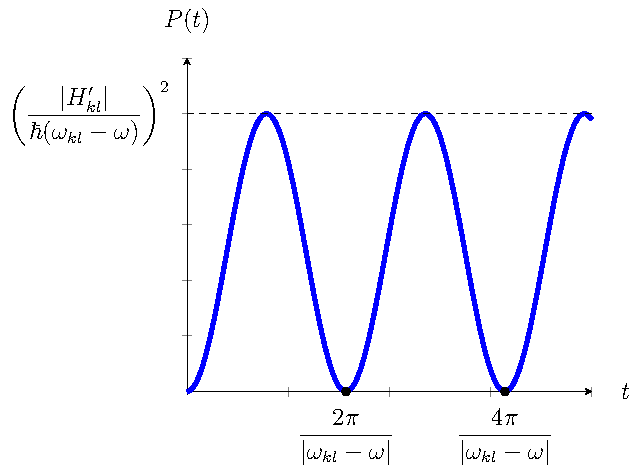
\includegraphics[width=0.51\linewidth]{absorption-t} \label{fig:prob-abs-t}}
	\subfloat[]{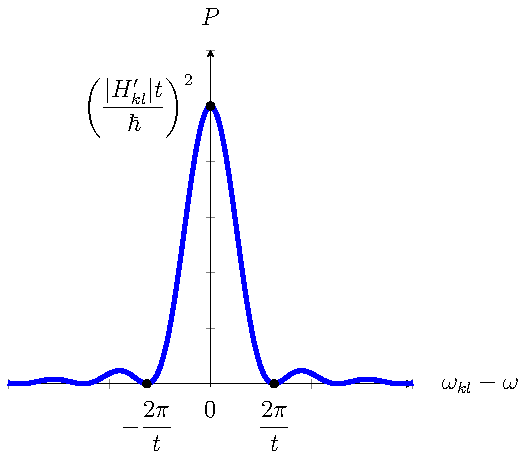
\includegraphics[width=0.46\linewidth]{absorption-w} \label{fig:prob-abs-w}}
	\caption{The transition probability from state $l$ to state $k$ plotted as \protect\subref{fig:prob-abs-t} a function of time, which displays oscillatory behavior with nodes at integer multiples of $2\pi/\abs{\omega_{kl}-\omega}$, and \protect\subref{fig:prob-abs-w} a function of frequency, which displays a sharp peak at $\omega=\omega_{kl}$ with width $4\pi/t$.}
	\label{fig:prob-abs}
\end{figure}

On the other hand, we see in Figure~\ref{fig:prob-abs-w} that in order to maximize the transition probability, the driving frequency $\omega$ should match the ``natural'' frequency $\omega_{kl}$. The peak has a finite width of $4\pi/t$ and becomes narrower and narrower as time progresses. Thus we see the manifestation of the uncertainty principle in the range of photon energies that are able to drive the transition. On a practical level, the complementarity between time and energy\footnote{Often expressed as $\Delta E \Delta t \ge \frac{\hbar}{2}$, or $\Delta \omega \Delta t \ge \frac{1}{2}$.} is something that we're probably familiar with. If we hear any note (frequency) for a very short amount of time, there is a lot of uncertainty as to what that note is. It's only when the note is extended that the true frequency of the sound wave is determined.

%%%%%%%%%%%%%%%%%%%%%%%%%%%%%%%%%%%%%%%%%%%%%%%%%%%%%%%%%%%%%%%%%%%%%%%%%%%%%%%%

\section{Application: Stimulated emission}
The precise control of the driving frequency to drive atomic transitions was leveraged by Charles Townes to construct the first \textbf{maser} (microwave amplification by stimulated emission of radiation) in 1953.\footnote{See this \href{https://physics.aps.org/story/v15/st4}{focus article} from \emph{Physics} about the history surrounding the maser and Townes' \href{https://journals.aps.org/pr/abstract/10.1103/PhysRev.99.1264}{original work}.} The maser was the precursor to the \textbf{laser}, which was invented seven years later and operates under the same principles to produce coherent radiation at visible wavelengths.\footnote{See T. H. Maiman \href{https://www.nature.com/nature/journal/v187/n4736/pdf/187493a0.pdf}{\emph{Nature}} \textbf{187} (1960).} \par

Both devices operate based on \textbf{stimulated emission}, which was predicted by Einstein back in 1917. Einstein knew that when photons of the right frequency strike an atom, the atom can ``absorb'' the photon and transition into a higher energy state (the electrons jump to higher energy levels). He then posited that it must be possible for the excited atom to return to a lower energy state by emitting a photon in a process known as \textbf{spontaneous emission}. Einstein, of course, did not stop there. He went one step further and postulated that if a photon of the right frequency encountered an excited atom, then there would be a probability that the photon will stimulate the excited atom to release a photon of identical frequency that traveled in the same direction. This process is illustrated in Figure~\ref{fig:laser}. Since we derived the probability of absorption in the text, we will leave it as an exercise to the reader to show that the probability of emission is in fact equivalent to Equation~\ref{eq:prob-abs}.

\begin{figure}[!h]
	\centering
	\subfloat[]{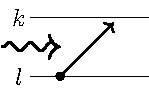
\includegraphics[width=0.20\linewidth]{absorption} \label{fig:absorption}} \qquad 
	\subfloat[]{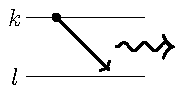
\includegraphics[width=0.23\linewidth]{spont-e} \label{fig:stimu-e}} \qquad 
	\subfloat[]{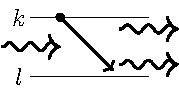
\includegraphics[width=0.22\linewidth]{stimu-e} \label{fig:spont-e}}
	\caption{The three ways in which light interacts with atoms include: \protect\subref{fig:absorption} Absorption, where a photon is absorbed by the atom and an electron transitions into an excited state. \protect\subref{fig:stimu-e} Spontaneous emission, where an excited atom emits a photon and an electron transitions to a lower energy state. \protect\subref{fig:spont-e} Stimulated emission, where an incident photon causes an excited atom to emit a coherent photon.}
	\label{fig:laser}
\end{figure}

Where stimulated emission becomes exciting is when we have a population inversion of many atoms in the excited state that all have the possibility of emitting coherent radiation. Then we get an \emph{amplification} effect where a single incident photon leads to two resulting photons, which then turn into four photons, and so on in a chain reaction. This is the basis for how masers and lasers function, and scientists are getting increasingly creative with these optical resonators. In particular, nanowire lasers, pioneered by Peidong Yang at UC Berkeley,\footnote{See M. H. Huang et al. \href{http://science.sciencemag.org/content/292/5523/1897.full}{\emph{Science}} \textbf{292}, 5523 (2001).} have recently attracted a lot of excitement in the world of nano-optics because they have demonstrated near 100\% efficiency---every single photon they absorb is used to produce a photon of laser light.\footnote{See H. Zhu et al. \href{http://www.nature.com/nmat/journal/v14/n6/full/nmat4271.html}{\emph{Nature Materials}} \textbf{14} (2015).}

%%%%%%%%%%%%%%%%%%%%%%%%%%%%%%%%%%%%%%%%%%%%%%%%%%%%%%%%%%%%%%%%%%%%%%%%%%%%%%%%

\section{Summary}
To recap, in this chapter we analyzed a quantum mechanical system where the Hamiltonian was no longer time-independent, thus exposing us to the framework of time-dependent perturbation theory. It turns out, however, that when the perturbation is small, we can employ our friendly eigenfunction expansion to arrive at a very good first order approximation for the exact solution. We looked at a particular case when the perturbation term is sinusoidal, which is an appropriate model for an electromagnetic field, and the transition probability we derived was sinusoidal in time as well. We finished with an analysis of stimulated emission, which is fundamental to the operation of the laser.

%} % for doublespacing
%\end{document}